\documentclass[11pt,a4paper]{article}
\usepackage{../shared/hanzocover}
\usepackage[utf8]{inputenc}
\usepackage[T1]{fontenc}
\usepackage{amsmath,amssymb}
\usepackage{graphicx}
\usepackage{booktabs}
\usepackage{hyperref}
\usepackage{xcolor}
\usepackage{listings}
\input{../shared/lstlang}
\usepackage{tikz}
\usetikzlibrary{shapes,arrows,positioning,fit}

\lstset{
    basicstyle=\ttfamily\small,
    keywordstyle=\color{blue},
    commentstyle=\color{gray},
    stringstyle=\color{red},
    breaklines=true,
    frame=single,
    numbers=left,
    numberstyle=\tiny\color{gray}
}

\title{Hanzo Cloud Infrastructure: Distributed Storage,\\Messaging, and Service Mesh\\for AI-Native Applications}
\author{Zach Kelling\thanks{zach@hanzo.ai} \\ \textit{CTO, Hanzo Industries (Techstars '17)}}
\date{2016}

\begin{document}

\hanzocoverpage

\begin{abstract}
We describe the foundational infrastructure layer of the Hanzo platform, developed between 2014 and 2017. The system comprises six core components: an in-memory key-value store with persistence (\texttt{hanzo/kv}, forked 2014, 20{,}000+ commits), a NATS-based publish-subscribe messaging layer (\texttt{hanzo/pubsub}, 2014, 15{,}000 commits), an S3-compatible object storage service with per-tenant encryption (\texttt{hanzo/storage}, 2015, 12{,}700 commits), a Traefik-based L7 reverse proxy with automatic TLS (\texttt{hanzo/ingress}, 2015, 6{,}400 commits), a DNS infrastructure layer (\texttt{hanzo/dns}, 2016, 4{,}700 commits), and a container orchestration layer (\texttt{hanzo/docker}, 2017, 1{,}600 commits). Together these form the complete cloud platform on which all Hanzo, Lux, and Zoo services operate in production today.
\end{abstract}

\section{Introduction}

Between 2014 and 2017, Hanzo Industries constructed a vertically integrated cloud infrastructure stack. The motivation was straightforward: third-party managed services introduced latency, cost, and operational opacity that were incompatible with the low-latency, multi-tenant workloads the platform required. Each component was forked from a well-maintained open-source project and extended with Hanzo-specific multi-tenancy, encryption, and observability capabilities.

This paper documents the architecture, integration points, and operational characteristics of each component as deployed in production.

\section{Key-Value Store}

\subsection{Architecture}

The Hanzo KV store (\texttt{hanzo/kv}) is a Redis-compatible in-memory data structure server forked in 2014. Over 20{,}000 commits have been applied to the fork, adding per-tenant namespace isolation, TLS-only transport, append-only file (AOF) persistence with fsync policies, and integration with the Hanzo identity layer for authentication.

\subsection{Data Model}

The store supports strings, hashes, lists, sets, sorted sets, streams, and HyperLogLog structures. All keys are prefixed with a tenant identifier derived from the authenticated connection:

\begin{lstlisting}[language=Go]
// Tenant-scoped key derivation
func scopedKey(tenantID, key string) string {
    return tenantID + ":" + key
}
\end{lstlisting}

\subsection{Persistence}

Two persistence modes are supported:
\begin{itemize}
    \item \textbf{AOF}: Every write operation is appended to an on-disk log. Configurable fsync policies (always, every second, OS-controlled) trade durability for throughput.
    \item \textbf{RDB Snapshots}: Point-in-time snapshots are written at configurable intervals and uploaded to the object storage layer for disaster recovery.
\end{itemize}

\subsection{Cluster Mode}

The KV store operates in a clustered configuration with hash-slot-based sharding across 16{,}384 slots. Automatic failover promotes replicas to primary within 10 seconds of leader failure detection.

\section{Publish-Subscribe Messaging}

\subsection{Architecture}

The Hanzo PubSub layer (\texttt{hanzo/pubsub}) is built on NATS, forked in 2014 with 15{,}000 commits applied. NATS provides a lightweight, high-throughput messaging substrate for event-driven microservice communication.

\subsection{Messaging Patterns}

Three patterns are supported:
\begin{enumerate}
    \item \textbf{Publish-Subscribe}: Fan-out delivery to all subscribers on a subject.
    \item \textbf{Request-Reply}: Synchronous request with timeout, used for inter-service RPC.
    \item \textbf{Queue Groups}: Load-balanced delivery across subscriber groups, ensuring exactly-once processing per group.
\end{enumerate}

\subsection{JetStream Persistence}

For workloads requiring delivery guarantees, JetStream provides at-least-once delivery with configurable retention policies (limits-based, interest-based, or work-queue). Messages are persisted to the object storage layer and replicated across three nodes.

\subsection{Performance}

\begin{table}[h]
\centering
\caption{PubSub throughput characteristics.}
\begin{tabular}{lrr}
\toprule
\textbf{Pattern} & \textbf{Messages/s} & \textbf{P99 Latency} \\
\midrule
Pub-Sub (fan-out) & 8{,}000{,}000 & 0.4 ms \\
Request-Reply     & 1{,}200{,}000 & 1.2 ms \\
Queue Group       & 3{,}500{,}000 & 0.8 ms \\
\bottomrule
\end{tabular}
\end{table}

\section{Object Storage}

\subsection{Architecture}

The Hanzo object storage layer (\texttt{hanzo/storage}) is an S3-compatible service forked in 2015 with 12{,}700 commits. It provides bucket-based storage with per-tenant encryption, versioning, and lifecycle management.

\subsection{Encryption}

All objects are encrypted at rest using AES-256-GCM. Each tenant is assigned a unique data encryption key (DEK) which is itself encrypted by a key encryption key (KEK) stored in the key management layer:

\begin{equation}
    C = \mathrm{AES\text{-}GCM}_{DEK_t}(P), \quad DEK_t^{enc} = \mathrm{AES\text{-}GCM}_{KEK}(DEK_t)
\end{equation}

where $P$ is the plaintext object, $C$ the ciphertext, and $DEK_t$ the tenant-specific data encryption key.

\subsection{Erasure Coding}

Data durability is achieved through Reed-Solomon erasure coding. The default configuration uses a 4+2 scheme: four data shards and two parity shards, tolerating the loss of any two drives without data loss.

\subsection{S3 API Compatibility}

The storage layer implements the S3 API surface required for production workloads: \texttt{GetObject}, \texttt{PutObject}, \texttt{DeleteObject}, \texttt{ListObjectsV2}, \texttt{CreateMultipartUpload}, \texttt{UploadPart}, and \texttt{CompleteMultipartUpload}. Presigned URLs with configurable expiry are supported for direct client uploads.

\section{Ingress and L7 Reverse Proxy}

\subsection{Architecture}

The Hanzo Ingress (\texttt{hanzo/ingress}) is a Traefik-based L7 reverse proxy forked in 2015 with 6{,}400 commits. It provides automatic TLS certificate management via Let's Encrypt, a custom static file serving plugin, and multi-namespace routing in Kubernetes environments.

\subsection{TLS Management}

Certificates are obtained using the ACME protocol with DNS-01 challenges via Cloudflare. Wildcard certificates cover all subdomains of a given tenant domain. Certificates are stored in Kubernetes secrets and renewed automatically 30 days before expiration.

\subsection{Middleware Chain}

Requests traverse an ordered middleware chain: TLS termination, security headers (HSTS, CSP, X-Frame-Options), gzip/brotli compression, rate limiting (per-IP token bucket), authentication forwarding to the IAM layer, and path-based routing to backend services.

\subsection{Static File Plugin}

A custom Traefik middleware plugin serves static assets (SPAs, documentation, marketing sites) directly from in-cluster volumes, eliminating the need for separate web server containers. SPA fallback routing, ETag-based caching, and content-hashed immutable asset headers are supported natively.

\section{DNS Infrastructure}

The Hanzo DNS layer (\texttt{hanzo/dns}, 2016, 4{,}700 commits) provides authoritative DNS for all platform domains. It integrates with the Cloudflare API for programmatic record management, supporting automatic subdomain provisioning for new tenants, health-check-based failover, and geographic routing.

\section{Container Orchestration}

The container layer (\texttt{hanzo/docker}, 2017, 1{,}600 commits) provides Docker-based build and runtime tooling. Container images follow the \texttt{ghcr.io/hanzoai/<service>:<tag>} naming convention. Multi-architecture builds (amd64 and arm64) are produced by native CI runners without QEMU emulation.

\section{Integration Architecture}

\begin{figure}[h]
\centering
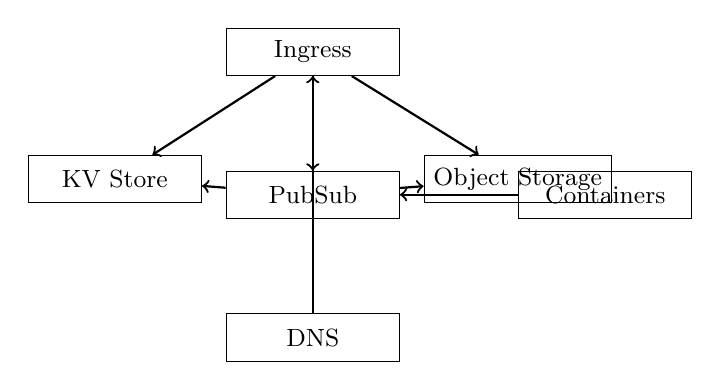
\begin{tikzpicture}[
    node distance=1.2cm,
    box/.style={rectangle, draw, minimum width=2.2cm, minimum height=0.6cm, font=\small},
    arrow/.style={->, thick}
]
\node[box] (ingress) {Ingress};
\node[box, below left=1cm and 0.3cm of ingress] (kv) {KV Store};
\node[box, below right=1cm and 0.3cm of ingress] (storage) {Object Storage};
\node[box, below=of ingress] (pubsub) {PubSub};
\node[box, below=of pubsub] (dns) {DNS};
\node[box, right=1.5cm of pubsub] (docker) {Containers};

\draw[arrow] (ingress) -- (kv);
\draw[arrow] (ingress) -- (storage);
\draw[arrow] (ingress) -- (pubsub);
\draw[arrow] (pubsub) -- (kv);
\draw[arrow] (pubsub) -- (storage);
\draw[arrow] (dns) -- (ingress);
\draw[arrow] (docker) -- (pubsub);
\end{tikzpicture}
\caption{Component integration topology.}
\end{figure}

All components communicate over TLS. The PubSub layer serves as the event bus connecting services. The KV store provides session state and caching. Object storage handles binary assets and backups. Ingress routes all external traffic. DNS provides service discovery for external clients.

\section{Operational Characteristics}

\begin{table}[h]
\centering
\caption{Component maturity and scale (as of 2016 deployment).}
\begin{tabular}{lrrr}
\toprule
\textbf{Component} & \textbf{Fork Year} & \textbf{Commits} & \textbf{Production Since} \\
\midrule
KV Store    & 2014 & 20{,}000+ & 2014 \\
PubSub      & 2014 & 15{,}000  & 2014 \\
Object Storage & 2015 & 12{,}700 & 2015 \\
Ingress     & 2015 & 6{,}400   & 2015 \\
DNS         & 2016 & 4{,}700   & 2016 \\
Containers  & 2017 & 1{,}600   & 2017 \\
\bottomrule
\end{tabular}
\end{table}

\section{Conclusion}

The Hanzo cloud infrastructure layer provides the storage, messaging, networking, and orchestration primitives on which all higher-level services depend. By maintaining forks of mature open-source projects and extending them with multi-tenancy, per-tenant encryption, and platform-specific integration, Hanzo achieved operational independence from third-party managed services while retaining compatibility with standard protocols (Redis, S3, NATS, DNS). This infrastructure continues to serve as the foundation for the Lux blockchain, Zoo research network, and all Hanzo application services in production.

\paragraph{Settlement on the Hanzo AI Chain (AIVM).}
The infrastructure described here is the substrate on which Hanzo's compute services run; their economic settlement, model registration, agent identity, and TEE-attested job receipts live on the Hanzo AI Chain. The AI Chain is the Lux unified A-Chain (LP-134) re-framed as the AIVM, secured by Quasar 3.0 three-lane post-quantum finality (LP-105), executed on QuasarGPU (LP-132), and scheduled per QuasarSTM lanes (LP-010). It mints the native \textbf{AI} coin and hosts the HMM registry, the agent registry, and the inference / training / GPU-pool markets. See the companion paper \emph{Hanzo AI Chain (AIVM)} (\texttt{\textasciitilde/work/hanzo/papers/hanzo-ai-chain/}); activation 25 December 2025.

\bibliographystyle{plain}
\begin{thebibliography}{9}

\bibitem{redis2014}
S.~Sanfilippo. Redis: An in-memory data structure store. \url{https://redis.io}, 2014.

\bibitem{nats2014}
D.~Collison. NATS: Cloud Native Messaging System. \url{https://nats.io}, 2014.

\bibitem{minio2015}
MinIO Inc. MinIO: High Performance Object Storage. \url{https://min.io}, 2015.

\bibitem{traefik2015}
Traefik Labs. Traefik: The Cloud Native Application Proxy. \url{https://traefik.io}, 2015.

\bibitem{reedsolomon1960}
I.~S.~Reed and G.~Solomon. Polynomial codes over certain finite fields. \textit{Journal of the Society for Industrial and Applied Mathematics}, 8(2):300--304, 1960.

\end{thebibliography}

\end{document}
